\documentclass{standalone}

\usepackage{tikz}

\begin{document}
  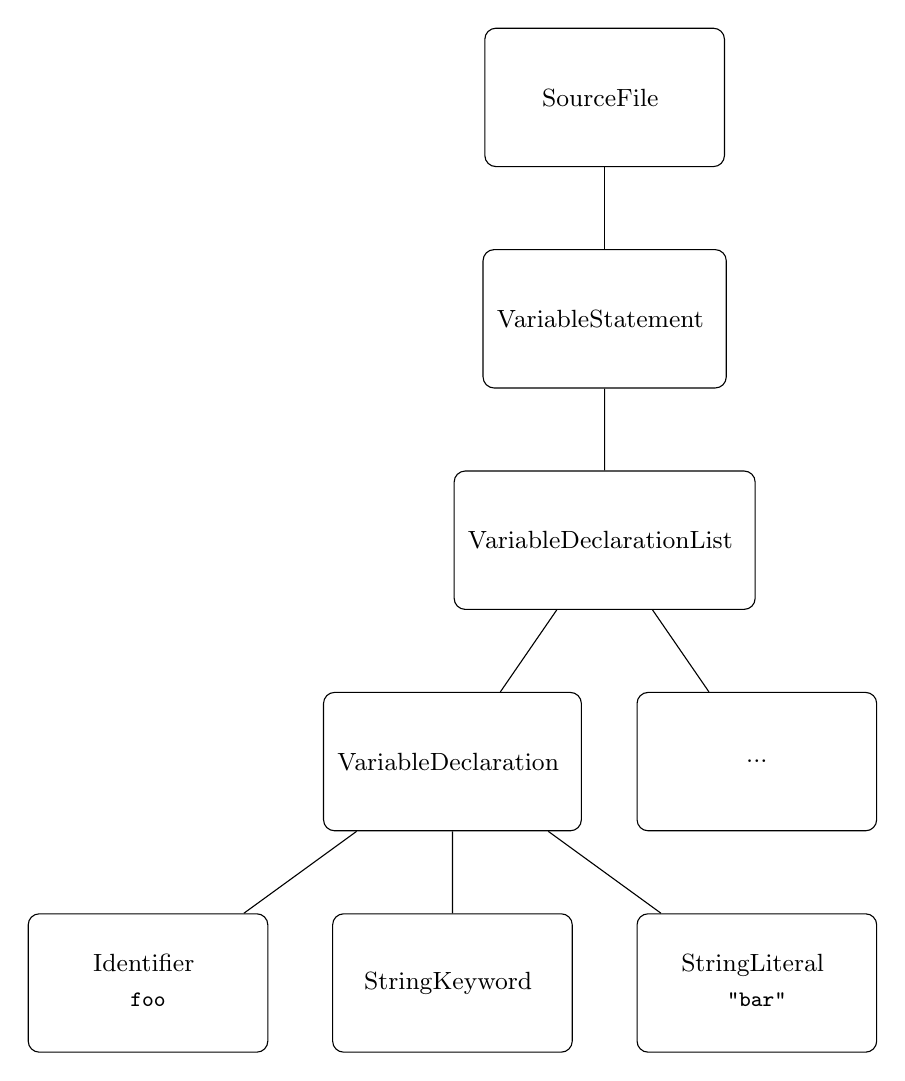
\begin{tikzpicture}[
    auto,
    sibling distance=11em,
    level distance=8em,
    font=\small,
    text centered,
    every node/.style = {
  	  minimum width=width("VariableDeclaration"),
  	  minimum height=5em,
      shape=rectangle,
  	  rounded corners,
  	  inner xsep=.5em,
      draw,
  	  align=center
  	}
    ]
    
    \node { SourceFile }
      child { node { VariableStatement }
  	  child { node { VariableDeclarationList }
  	    child { node { VariableDeclaration }
  		  child { node { \begin{tabular}{c}Identifier \\[.2em] \footnotesize{\texttt{foo}}\end{tabular} } }
  		  child { node { StringKeyword } }
  		  child { node { \begin{tabular}{c}StringLiteral \\[.2em] \footnotesize{\texttt{"bar"}}\end{tabular} } }
  		}
  		child { node {...} }
  	  }
  	};

  \end{tikzpicture}
\end{document}
